El resultado mas prometedor no es una clasificacion final de planetas, sino la identificacion de grafos y regiones candidatos para inspeccion cientifica. En esta corrida, el espacio orbital PCA es prioritario porque combina estructura no trivial con baja dependencia de imputacion. El espacio termico es topologicamente complejo, pero debe tratarse con cautela por su alta fraccion de imputacion. La inclusion de densidad derivada reduce ligeramente la complejidad de Mapper, lo que sugiere que \texttt{pl\_dens} actua como coordenada regularizadora mas que como fuente independiente de nueva ramificacion. \begin{figure}[H]\centering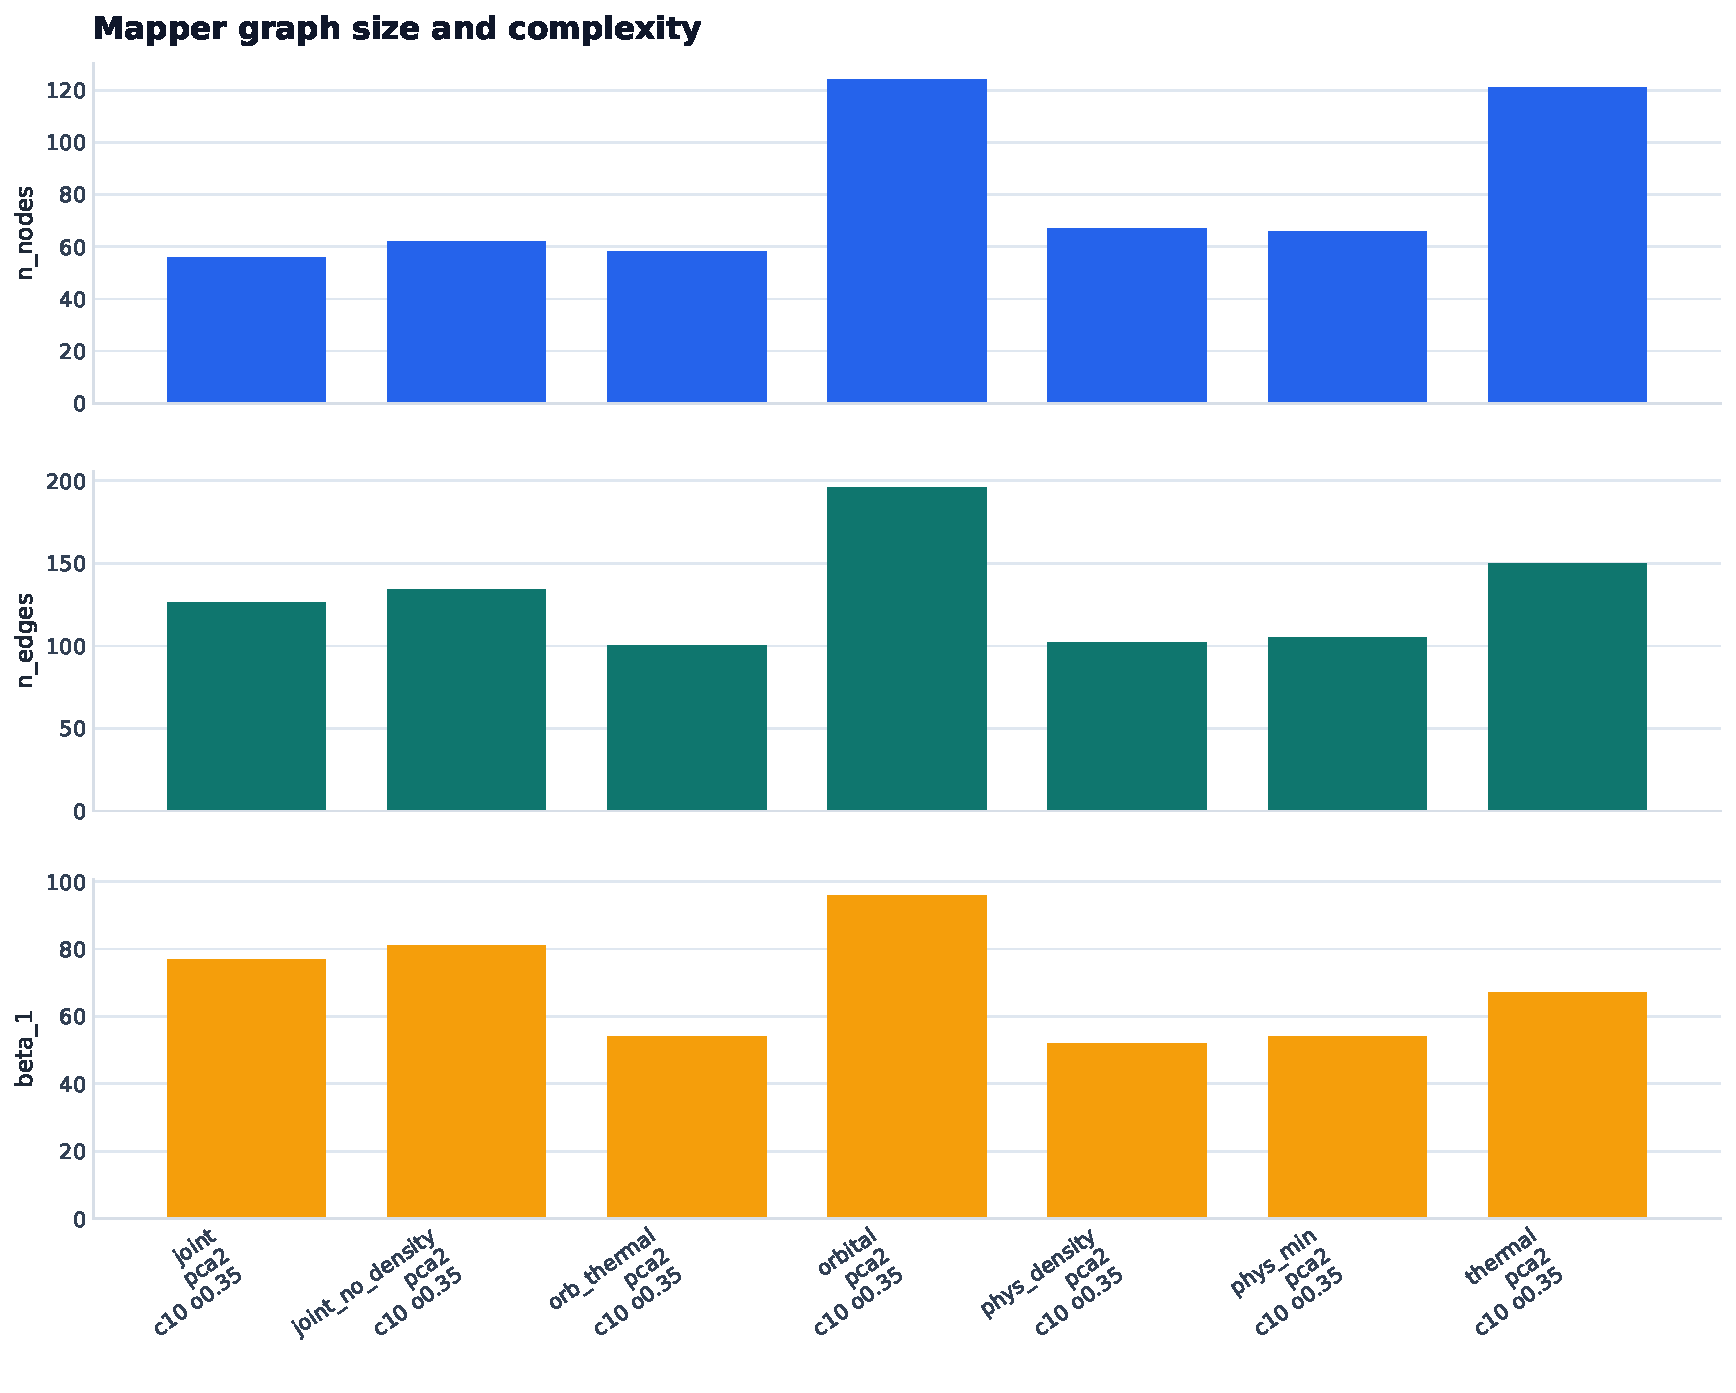
\includegraphics[width=0.95\linewidth]{figures/01_mapper_graph_size_complexity.pdf}\caption{Tamano y complejidad de los grafos Mapper.}\end{figure}\begin{figure}[H]\centering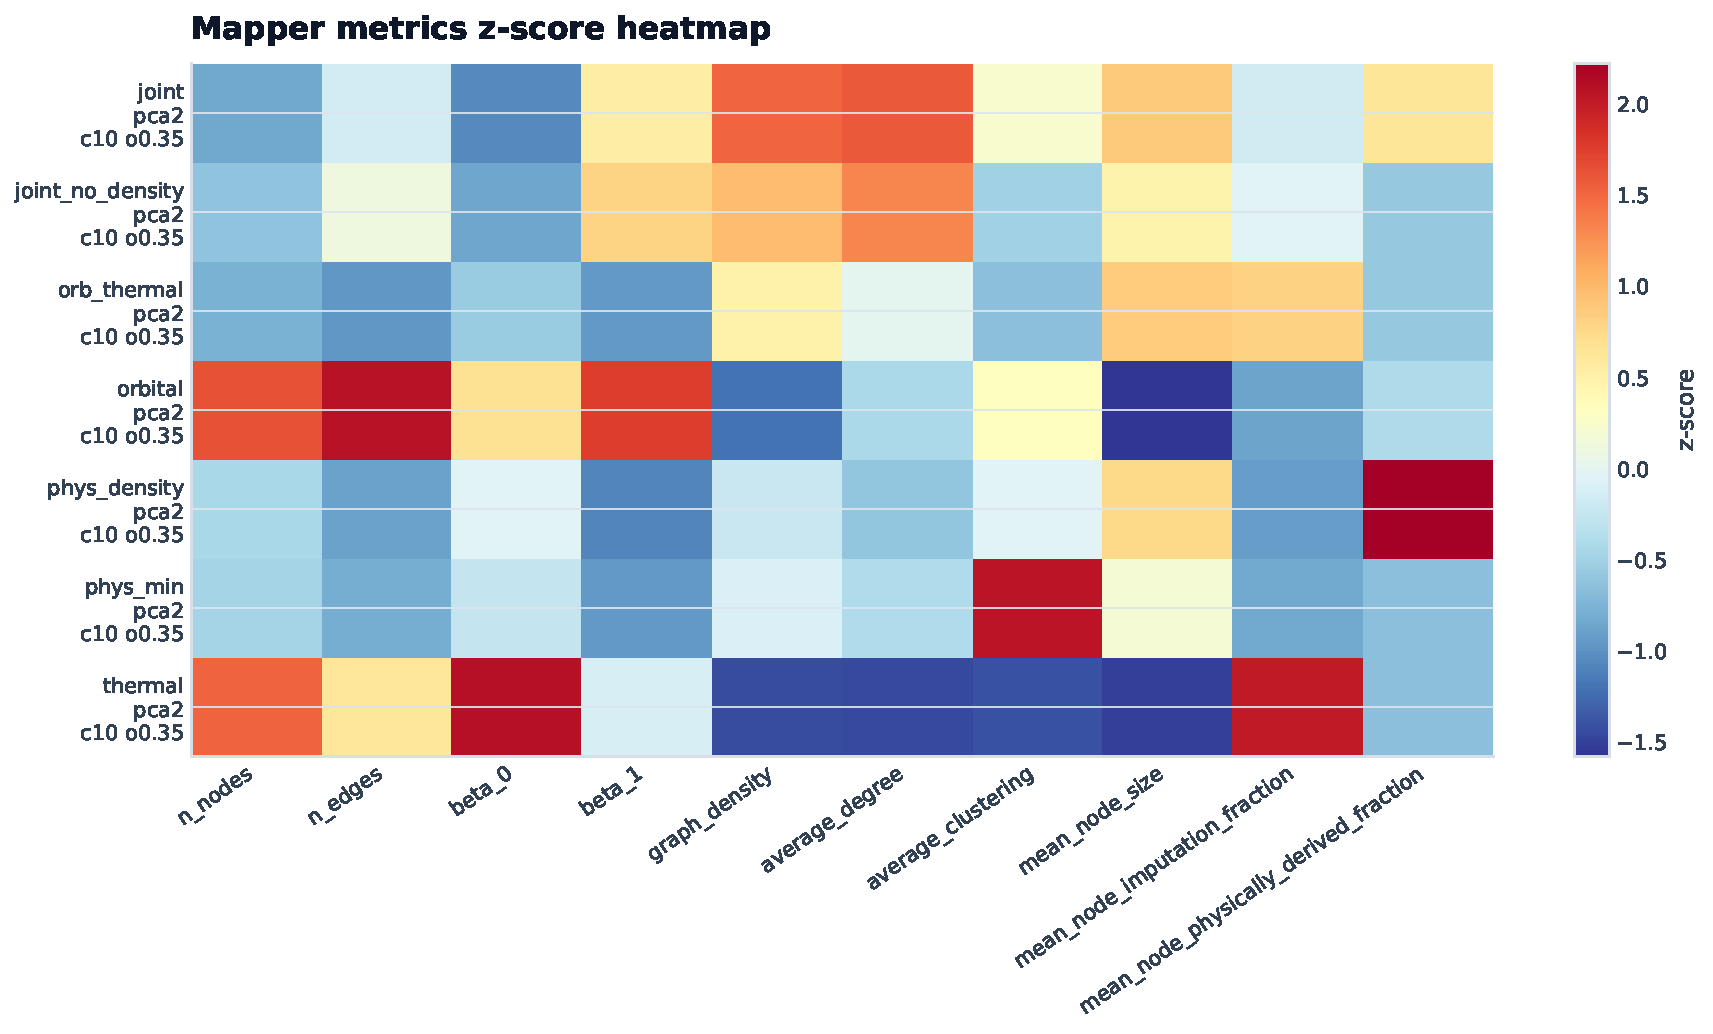
\includegraphics[width=0.95\linewidth]{figures/02_mapper_metrics_zscore_heatmap.pdf}\caption{Heatmap de metricas estandarizadas.}\end{figure}\begin{figure}[H]\centering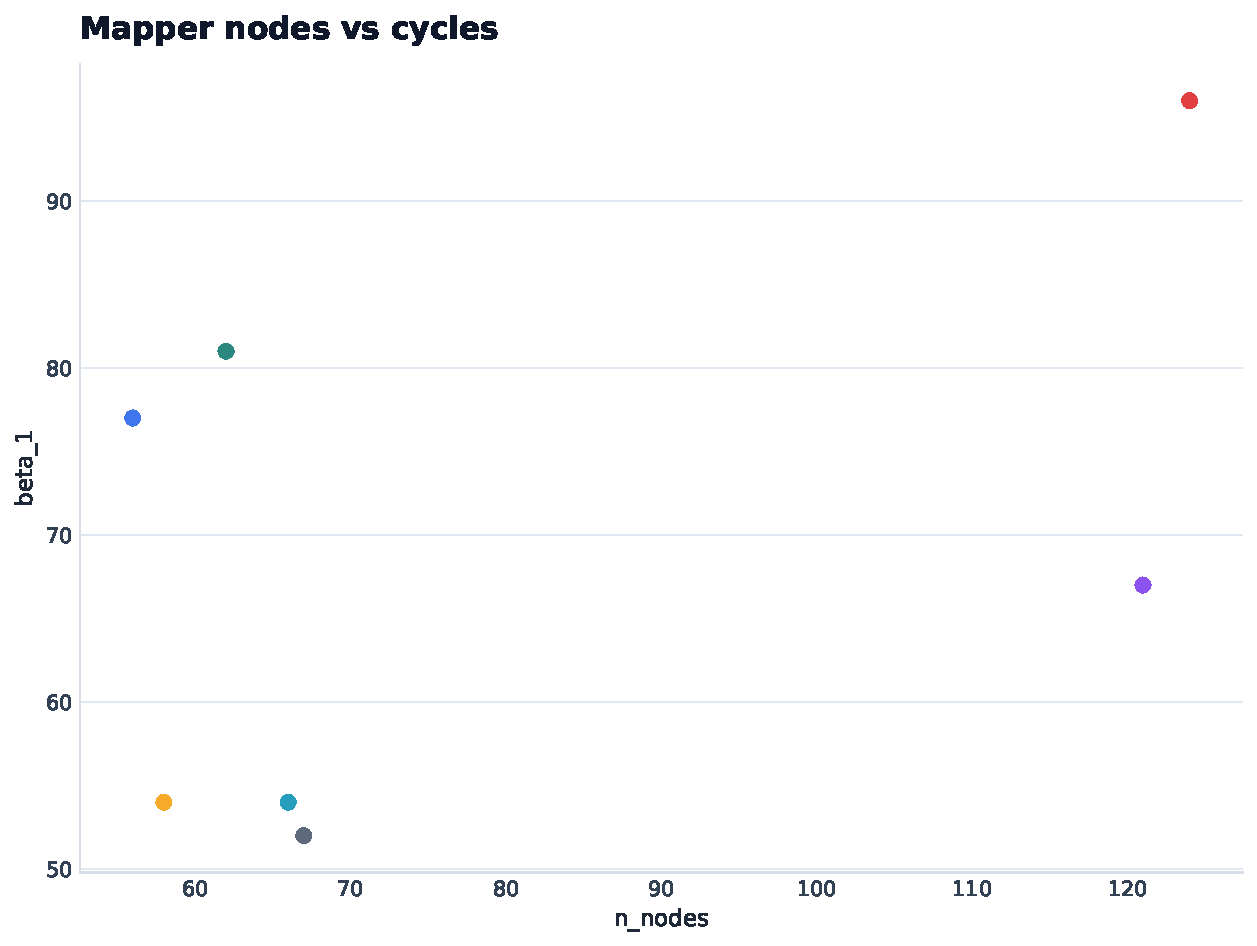
\includegraphics[width=0.75\linewidth]{figures/04_mapper_nodes_vs_cycles.pdf}\caption{Relacion entre numero de nodos y ciclos.}\end{figure}
